\titledquestion{Minimum Spanning Tree}
Consider the following weighted undirected graph.
\begin{center}
  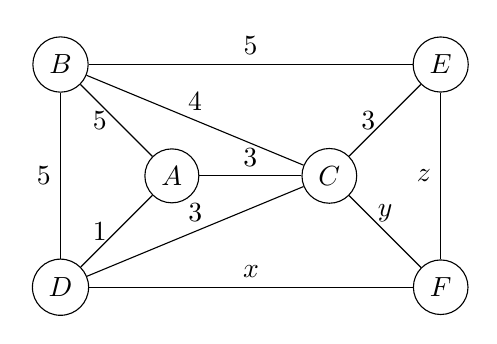
\begin{tikzpicture}[node distance = 2cm]
    \node[draw, circle] (B) {\fns\(B\)};
    \node[draw, circle, below right of = B] (A) {\fns\(A\)};
    \node[draw, circle, below left of = A] (D) {\fns\(D\)};
    \node[draw, circle, right of = A] (C) {\fns\(C\)};
    \node[draw, circle, above right of = C] (E) {\fns\(E\)};
    \node[draw, circle, below right of = C] (F) {\fns\(F\)};
    \foreach \i\j\k in {B/E/5, B/C/4, A/C/3, C/D/3, C/F/y, D/F/x} {
      \draw[] (\i) edge node[above] {\(\k\)} (\j);
    }
    \foreach \i\j\k in {A/B/5, A/D/1, C/E/3} {
      \draw[] (\i) edge node[left] {\(\k\)} (\j);
    }
    \draw[] (B) edge node[left] {\(5\)} (D);
    \draw[] (E) edge node[left] {\(z\)} (F);
  \end{tikzpicture}
\end{center}
\begin{parts}
  \part[3] Suppose \((x,y,z)=(4,1,2)\) and that we use the Kruskal's algorithm to find a minimum spanning tree of the graph. To make your answer unique and clear, please follow the rules below.
  \begin{itemize}
    \item Use \((u,v)\) to represent an undirected edge \(\{u,v\}\), where \(u<v\).
    \item Edges with same weight are sorted in alphabetical order. If two edges \(e_1=(u,v)\) and \(e_2=(w,t)\) have the same weight, \(e_1\) appears before \(e_2\) in the edge list if \((u<w)\lor\left((u=w)\land(v<t)\right)\).
  \end{itemize}
  Write down the sequence of edges added into the minimum spanning tree, and draw the tree.
  \begin{solution}
    %\vspace{2in}
    \\$(A,D)$\\
    $(C,F)$\\
    $(E,F)$\\
    $(A,C)$\\
    $(B,C)$\\

    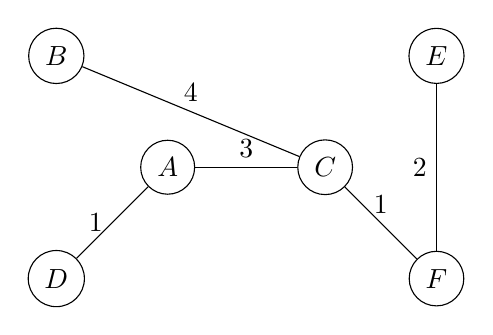
\begin{tikzpicture}[node distance = 2cm]
      \node[draw, circle] (B) {\fns\(B\)};
      \node[draw, circle, below right of = B] (A) {\fns\(A\)};
      \node[draw, circle, below left of = A] (D) {\fns\(D\)};
      \node[draw, circle, right of = A] (C) {\fns\(C\)};
      \node[draw, circle, above right of = C] (E) {\fns\(E\)};
      \node[draw, circle, below right of = C] (F) {\fns\(F\)};
      \foreach \i\j\k in {B/C/4, A/C/3, C/F/1} {
        \draw[] (\i) edge node[above] {\(\k\)} (\j);
      }
      \foreach \i\j\k in {A/D/1} {
        \draw[] (\i) edge node[left] {\(\k\)} (\j);
      }
      \draw[] (E) edge node[left] {\(2\)} (F);
    \end{tikzpicture}
    
  \end{solution}
  \part[3] If \((x,z)=(2,3)\), for what values of \(y\) is the edge \(\{C,F\}\) guaranteed to be contained in a minimum spanning tree? Give a sufficient and necessary condition and briefly justify your answer.
  \begin{solution}
    %\vspace{1in}
    \\
    the sufficient and necessary condition is $y < 3 $\\
    proof:\\
    cosider the cycle made up by the edges $(C,D),(C,F),(D,F)$
    the edge with biggest weight must not be in the MST, so we have to make sure $y$ is not the biggest weight in the cycle.
    and since $weight(C,D)=3,wight(D,F)=x=2$, so $y < 3$\\
    similarly, cosider the cycle made up by the edges $(C,E),(C,F),(E,F)$
    the edge with biggest weight must not be in the MST, so we have to make sure $y$ is not the biggest weight in the cycle.
    and since $weight(C,E)=3,wight(E,F)=z=2$, and $(C,F) must be in the cycle, $so $y < 3$\\
    so above all, the values of $y$ is $y < 3$.

  \end{solution}
  \part[2] If \(5\notin\{x,y,z\}\), is it possible for an edge weighted \(5\) to appear in a minimum spanning tree? Briefly justify your answer.
  \begin{solution}
    %\vspace{1in}
  \\
  It is impossible.\\
  proof:\\
  we can make the graph into two partitions.\\
  one set is \{A,B,C,D,E\}, and the other one is \{F\}\\
  for the first set, there exist an unique MST combined with edges \\$(A,C),(A,D),(B,C),(C,E)$
  and there weights are $1,3,4,3$, so the MST for the first set do not include edge weighted $5$.\\
  since the second set only include one vertex, so we do not need to consier its MST.\\
  to connected the two sets, and generate the MST of the whole graph, we need to take some edges which are connecting two sets.\\
  which means we will take the some of the weights in \{x,y,z\}.\\
  and since \(5 \notin \{x,y,z\}\), so the wight(s) we will take $\neq 5$\\
  so above all, it is impossible to have an edge weighted $5$ in the MST.

  \end{solution}
\end{parts}